\newpage
\section{Aufbau und Funktionsweise}
	
	\begin{wrapfigure}{r}{0.6\textwidth}
		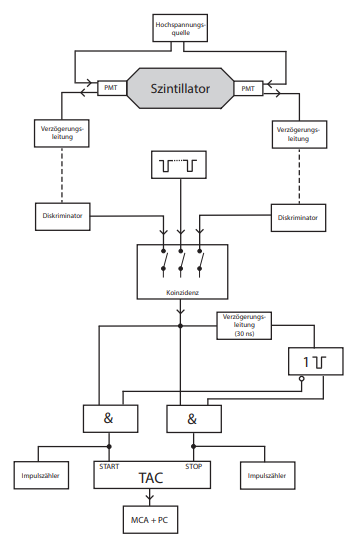
\includegraphics[width=10cm]{latex/images/Aufbau.png}
		\caption{Skizze der Schaltung \cite{Versuch}}
		\label{fig:Aufb}
	\end{wrapfigure}
    In Abbildung \ref{fig:Aufb} ist die in diesem Versuch verwendete Schaltung gezeigt.
    Diese Schaltung wird genutzt um zu erkennen wie viele Myonen in dem Messzeitrum in den Messkörper eintreten, wie viele dieser eingetreten Myonen innerhalb des Körpers zerfallen und wie viel Zeit zwischen dem Einfall und Zerfall liegt.
    Der Messkörper ist ein organischer Szintillationstank mit einem Volumen von ungefähr 50 Litern.
    Beim Eintreten der Myonen in den Detektor, werden die Myonen abgebremst und erzeugen einen Lichtblitz.
    Zerfällt das Myon innerhalb des Detektors, entsteht ein hochenergetisches Elektron welches wiederum wieder mit dem Szintillatormaerial wechselwirkt und einen Lichtblitz erzeugt.
    Zur Messung dieser Signale, sind an beiden Enden des Tanks Photomultiplier(PMT) angebracht, diese wandeln das eingehende Lichtsignal in einen Spannungsimpuls um. 
    Die PMT sind zur Rauschunterdrückung, zunächst über einen Verzögerungsleiter, an Diskriminatoren angebracht.
    Diese dienen dazu den Großteil der thermischen Anregungen der PMT auszufiltern, welche niederenergetischer sind als die Myonen Signale.
    An den Diskriminatoren wird eine gewisse Schwellspannung $U_0$ eingestellt, damit möglichst viele Rauschsignale unterdrückt werden aber auch möglichst keine echten Signale verloren gehen.
    Weitergehend werden hochenergetische thermische Anregungen der PMT ausgefiltert, indem beide Diskriminatoren an eine Koinzidenzschaltung angeschlossen werden.
    Die Koinzidenzschaltung gibt nur ein Signal weiter, wenn beiden eingehenden Signale innerhalb eines Zeitraumes $t_k$ eintreffen. 
    Mit diesen beiden Filtermethoden können die unkorrelierten Störungen nur mit einer sehr geringen Wahrschleinlichkeit ein echtes Signal erzeugen.
    Jetzt folgt der Schaltungsteil der zählt wie viele Signale entstehen und falls das Myon innerhalb des Detektors zerfällt, wie lange es gelebt hat.
    Dies erfolgt indem das Outputsignal der Koinzidenzschaltung in 3 Signale aufgeteilt wird.
    Zwei dieser Signale werden jeweils an eine Seite eines AND- Gatters angeschlossen, das Dritte wird mit einer Verzögerung von ca. $\SI{30}{\nano\second}$ an einen Monoflop angeschlossen.
    Der Monoflop gibt nach dem er durch ein HIGH Signal getriggert wurde für eine gewisse einstellbare Zeit $t_s$ ein HIGH Signal aus, dies ist die Suchzeit $t_s$ in der beobachtet wird ob das Myon zerfällt.
    Der Output des Monoflops ist nun invertiert an dem 1. AND-Gatter und normal an dem 2. AND-Gatter angeschlossen.
    Wenn die Schaltung im Ruhezustand ist und das Signal eines eintretenden Myon ankommt, liegen an dem ersten AND-Gatter nun zwei HIGH Signale, da durch die Verögerung, der Monoflop noch nicht aktiviert wurde.
    Dieses HIGH Signal wird an einen Impulszähler weitergegeben und startet den Zeit-Amplituden-Converter(TAC).
    Am Zweiten AND-Gatter liegen aufgrund der Verzögerung jedoch ein HIGH und LOW Signal.
    Wenn das Myon jetzt jedoch innerhalb der Suchzeit $t_s$ zerfallen ist und ein weiteres Signal erzeugt, verhält sich die Schaltung anders.
    Jetzt liegt durch den Monoflop noch ein LOW Signal am ersten AND-Gatter an, der erste Impulszähler und der Zeit-Amplituden-Converter werden nicht erneut aktiviert.
    An dem zweiten AND-Gatter liegen dann jedoch zwei HIGH-Signale an, dieses ist an einen Impulszähler und an den Zeit-Amplituden-Converter angeschlossen und stoppt diesen.
    Der Zeit-Amplituden-Converter gibt nun ein Signal mit einer Spannungshöhe korreliert zu der Zeitlänge an einen Multi-Channel-Analyser(MCA) weiter, welches von einem PC ausgewertet wird.

\section{Durchführung}
	
	Zunächst wird die Schaltung nach Abbildung \ref{fig:Aufb} aufgebaut, dazu müssen die verschiedenen Schaltungskomponente korrekt aneinander geschalten werden.
	Dann folgt die Justierung der Schaltung, dazu wird neben den Messgeräten des Versuches ein Oszilloskop verwendet.
	Zunächst werden die Schwellspannungen an den Diskirminatoren so eingestellt, dass auf beiden Seiten eine Signalrate von ca. $\SI{30}{\hertz}$ anliegt. 
    Dann werden die Einstellungen der Verzögerungsleiter bei einer Pulsdauer von $\Delta t= \SI{20}{\nano\second}$ und $\Delta t= \SI{10}{\nano\second}$ optimiert.
	Die Pulsdauern werden an den Diskriminatoren über kleine Schrauben verändert und an dem Oszillospkop abgelesen.
	Nun werden beide Diskirimnatoren an die Koinzidenzschaltung geschalten, je einer der Verzögerungsleiter verstellt und die Signalrate gemessen.
	Durch systematisches, einzelnes Verstellen der Verzögerungen ergibt sich eine Kurve der Signalraten, es sollten genug Werte aufgenommen werden um die Halbwertsbreite dieser Kurve zu bestimmen.
	Jetzt wird für den restlichen Versuch bei einer Signallänge von $\Delta t= \SI{10}{\nano\second}$ die optimale Verzögerung eingestellt, es sollte eine Ereignissrate von $\SI{20}{\hertz}$ anliegen.
	Weiterhin wird der TAC so eingestellt, dass möglichst viele Kanäle des MCA genutzt werden.
	Dazu wird der Doppelpulsgenerator mit einem Impulsabstand von $\SI{10}{\nano\second}$ an die Koinzidenzschaltung geschalten und der TAC so eingestellt, dass ein Channel in der Mitte angesprochen wird.
	Zuletzt wird noch der TAC und MCA so kalibriert, dass aus der Spannungshöhe bzw. dem Channel eine Lebensdauer berechnet werden kann.
	Dazu wird wieder der Doppelpuls generator an die Koinzidenzschaltung angeschlossen, 10 unterschiedliche Impulsabstände eingestellt und jeweils der Channel vermessen.
	Mit den Informationen der Channel und der Impulsabstände lässt sich der TAC und der MCA kalibrieren.

